\documentclass[12pt]{article}
\usepackage{axioma}
\usepackage{amsmath}
\begin{document}
\title{Implementation of convertible bond pricer with credit risk using PDE model}
\author{Zheng Gao}
\date{}
\maketitle

\section{Introduction\label{sec:intro}}
Convertible bonds ($CB$) have been around for more than a century. It is a security in which the investor can convert the instrument into a predefined number of shared of the company that issued the bond. The conversion is not mandatory and is an option for the investor. At maturity, the holder has the right to swap the face value $F$ of the bond for $C_r$ shared with price $S$, where $C_r$ is the conversion ratio. Most convertibles are American-style in their conversion possibilities: converting the bond into shares is not limited to the maturity date only, but may happen during a predefined conversion period. In addition to conversion feature, there is also a possibility for the bond to be called by the issuer in time interval $\Omega_{call}$ and to be put by the investor in time interval $\Omega_{put}$. The moment the bond gets called, the investor can sill convert into shares even not in the conversion interval. 

The difficulty for solving the Black-Scholes equation for $CB$ is that one can hardly assign a predetermined value to the credit spread $r_c$. If the easily observable credit spread implied by a similar non-convertible bond of the same issuer were used for $r_c$, one would unnecessarily penalize the risk-free equity upside of the CB.

An feasible numerical method was proposed by \textit{Tsiveriotis} and \textit{Fernandes}, who defined a related security, that is the "cash-only" part of the $CB$ and we will refer to as $COCB$. The price of $COCB$ is a derivative of the stock $S$, and thus should follow the Black-Scholes equation as does the $CB$ value. This leads to a new formulation of the $CB$ valuation problems as a system of two coupled Black-Scholes equation:
\begin{equation}
CB: \frac{\partial{U}}{\partial{t}} + 
\frac{\sigma^2S^2}{2}\frac{\partial^2{U}}{\partial{S}^2} + r_gS\frac{\partial{U}}{\partial{S}} - r(U-V) - (r+r_c)V + f(t) = 0 
\label{eq:CB}
\end{equation}

\begin{equation}
COCB: \frac{\partial{V}}{\partial{t}} + 
\frac{\sigma^2S^2}{2}\frac{\partial^2{V}}{\partial{S}^2} + r_gS\frac{\partial{V}}{\partial{S}} - (r+r_c)V + P(t) = 0 
\label{eq:COCB}
\end{equation}
where $U$ is the value of $CB$, $V$ is the value of $COCB$; $r_c$ here becomes the observable credit spread implied by the non-convertible bonds of the same issuer for $CB$; $S$ is the price of the underlying stock; $r$ is the risk-free rate; $r_g$ is the growth rate of the stock; $\sigma$ is the volatility and $P(t)$ denotes the bond paying coupons $c_i$ at $t_i$:
\begin{equation}
P(t) = \Sigma c_i\delta(t-t_i)
\label{eq:coupon}
\end{equation}
where $\delta(x)$ is the Dirac function, that is $\delta(x)$ equals to $1$ at $x = 0$ and equal to $0$ elsewhere.

The final condition as well as the boundary constraints are defined below:
\begin{itemize}
\item Final conditions at maturity:
\begin{eqnarray}
U = C_r S, V = 0\text{, if } S \ge F/C_r\\
U = F + c_{last}, V = F + c_{last}\text{, elsewhere }
\end{eqnarray}
where $c_{last}$ is the last coupon payment.

\item Upside constraints due to conversion at any time:
\begin{eqnarray}
U \ge C_r S\\
V = 0 \text{, if } U \le C_r S
\end{eqnarray}

\item Upside constraints due to callability by the CB issuer when $t\in \Omega_{call}$:
\begin{eqnarray}
U \le \max(B_{call}, C_rS)\\
V = 0 \text{, if } U \ge B_{call}
\end{eqnarray}

\item Downside constraints due to putability by the investor when $t \in \Omega_{put}$:
\begin{eqnarray}
U \ge B_{put} \\
V = B_{put} \text{, if } U \le B_{put}
\end{eqnarray}
 
\end{itemize}

The quoted price are usually the clean price, and thus the dirty call price and dirty put price are given by including any accruded interest that has accumulated since last coupon payment:
\[B_{call} = B_{call}^{clean} + AccI(t)\]
\[B_{put} = B_{put}^{clean} + AccI(t)\]
where $AccI(t)$ is the accruded interest at time equal to $t$ between $t_k^c$ and $t_{k+1}^c$:
\[
AccI(t) = c_k\frac{t-t_k^c}{t_{k+1}^c - t_k^c}
\]
where $c_k$ is the coupon payment at the $k$-th pay time $t_k^c$.

\section{Numerical Scheme}
\subsection{Discretization}
Notice that Equation \ref{eq:CB} and \ref{eq:COCB} are derived for American-style derivatives, and therefore results in a set of fully coupled free-boundary problems. Although Equation \ref{eq:COCB} appears to be independent of Equation \ref{eq:CB}, they are actually tightly coupled to each other due to the free boundaries introduced by $CB$ and Equation \ref{eq:CB} and \ref{eq:COCB} are not valid beyond these boundaries. To solve these fully coupled parabolic equations with free boundaries, Equation \ref{eq:CB} and \ref{eq:COCB} are firstly discretized using common numerical schemes, such as Forward in Time Centered in Space (FTCS), Backward in Time Centered in Space (BTCS) and semi-implicit Crank-Nicholson(CN) scheme. Then the resulting linear system is solved with Projected Successive Over-relaxation (PSOR) method by considering the conversion, puttability and callability during each iteration step. To simplify the implementation, we gives the discretized form for a generalized B-S equation:
\begin{equation}
\frac{\partial{U}}{\partial{t}} + 
c_2S^2\frac{\partial^2{U}}{\partial{S}^2} + c_1S\frac{\partial{U}}{\partial{S}} + c_0U + f(t) = 0 \label{eq:BS}
\end{equation}
where $U$ is the unknown solution, $c_2$ is the coefficient for second order term, $c_1$ for the first order term, $c_0$ for the zero order term, and $f(t)$ denotes the source term to the PDE. Let $U^n_i$ denote numerical solution to Equation \ref{eq:BS} at $S = S_i = S_0 + i \Delta S$ and $t = t_n = t_0 + n \Delta t$, the discretized form is derived as:
\begin{eqnarray*}
[1 + (\alpha_{i}+\beta_{i} - c_0 \Delta t)\theta] U_i^n 
- (\alpha_i U_{i-1}^n + \beta_i U_{i+1}^n)\theta \\
= [1 - (\alpha_i+\beta_i - c_0 \Delta t)(1-\theta)] U_i^{n+1} 
+ (\alpha_i U_{i-1}^{n+1} 
+ \beta_i U_{i+1}^{n+1})(1-\theta) + f_i \Delta t
\end{eqnarray*}
where
\begin{eqnarray}
\alpha_i = (\frac{c_2S_i^2}{\Delta S^2} - \frac{c_1S_i}{\Delta S})\Delta t\\
\beta_i =  (\frac{c_2S_i^2}{\Delta S^2} + \frac{c_1S_i}{\Delta S})\Delta t
\end{eqnarray}
The parameter $\theta$ is used to generalize to different schemes, $\theta = 0$ for FTCS, $\theta = 1$ for BTCS and $\theta = 0.5$ for CN method. Since the equation is solved backwards from maturity, the above equation is solved for $U^{n}$ from $U^{n+1}$. Note that although the above formula is derived based on the uniform mesh grid, we have used the varied grid size in the implementation.

\subsection{Boundary Conditions}
The boundary condition significantly affect the solution of the PDE. The discretized form corresponding to lower and upper boundary is described as follows:

When $S = 0$, we assume $\alpha_i = 0$, $\beta_i = 0$. This yields that
\begin{equation}
(1 - c_0\theta\Delta t)U_i^n = [1+c_0(1-\theta\Delta t)]U_{i+1}^{n+1} + f_i^{n+1}\Delta t
\end{equation}

When $S$ is large, only the second order term remains in the equation, and hence we have
\begin{equation}
U_{i+1}^n + U_{i-1}^n - 2 U_{i}^n = 0
\end{equation}

\subsection{Linear System}
The above formulas result in a tridiagonal linear system to be solved at every time step:
\begin{equation}
(\mathbf{I} + \theta \mathbf{M}) \mathbf{U}^{n} = (\mathbf{I} - (1-\theta)\mathbf{M})\mathbf{U}^{n+1} + \mathbf{f}^{n+1}\Delta t
\end{equation}
where
\begin{equation}
\mathbf{M} = 
\begin{bmatrix}
-c_0\theta\Delta t         & 0        & 0 		  & \dots & 0\\
-\alpha_1 & \alpha_1 + \beta_1 - c_0\Delta t & -\beta_1 & \dots & 0\\
0         & -\alpha_2  & \alpha_2 + \beta_1 - c_0\Delta t & \dots & 0 \\                 
\vdots & \vdots & \vdots & \ddots & -\beta_{m-1} \\
0 & 0 & 0 & \dots & 0
\end{bmatrix}
\end{equation}
For the equation of CB, $c_2 = \sigma^2/2$, $c_1 = r_g$, $c_0 = -r$ and $\mathbf{f} = -r_c \mathbf{V}$, and for COCB, $c_2 = \sigma^2/2$, $c_1 = r_g$, $c_0 = -(r+r_c)$ and $\mathbf{f} = \mathbf{0}$. In consideration of efficiency, only the tridiagonal band part of the coefficient matrix is stored and send to the the PSOR solver.  

\subsection{Projected Successive Over-relaxation Method}
The PSOR iteration is used to solve the problem of $\mathbf{Ax} = \mathbf{b}$ with constraints, where $\mathbf{A} = (\mathbf{I} + \theta M)$ and $ \mathbf{b} = (\mathbf{I} - (1-\theta)\mathbf{M})\mathbf{U}^{n+1} + \mathbf{f}\Delta t$. Here we use $\mathbf{I}$ to represent identity matrix, $a_{ij}$ to represent the $i$th-row, $j$th-column element in matrix $\mathbf{A}$, and $b_i$ to represent the $i$-th element in vector $\mathbf{b}$. For each $x^k_i$ in the solution space at the $k$-th iteration, the recursion formula is:
\begin{equation}
x_i^{k+1} = (1-\omega)x_i^{k} + \frac{\omega}{a_{ii}}(b_i - \Sigma_{j < i} a_{ij}x_{j}^{(k+1)} - \Sigma_{j > i}a_{ij}x_j^{k})
\end{equation}
where $0< \omega < 2$ is the relaxation factor. The iteration terminates when the number of iterations exceeds a preset number or the $2$-norm of the difference of the solution at the $k$-th and $k+1$-th step is smaller than the preset tolerance.

After each iteration step, the constraints in section \ref{sec:intro} are applied once to the solution space. In specific, the upside and downside constraints are applied as follows:
\begin{itemize}
\item
If $U_i > \max(B_{call}, C_rS_i)$ and $t\in \Omega_{call}$, let
\[U_i = \max(B_{call}, C_rS_i)\]
\[V_i = 0\]
\item
If $U_i < B_{put}$ and $t\in \Omega_{put}$, let
\[U_i = B_{put}\]
\[V_i = B_{put}\]
\item
If $U_i < C_rS_i$, let
\[U_i = C_rS_i\]
\[V_i = 0\]
\end{itemize}
Without loss of generality, when the CB is not puttable, we can set $B_p = 0$, and, when it is not callable, we set $B_c = \infty$. 

\subsection{Coupon Payments}
Consider the discrete time point $t_n$ before coupon pay time $t_c$ and $t_{n+1}$ after coupon pay time $t_c$. If such a $t_c$ exists, the time stepping size $dt$ must be reduced to $t_{n+1} - t_c$. Then the discrete coupon payments are handled by adding the coupon payment to the solution:
\[\mathbf{U}^{n+1} = \mathbf{U}^{n+1} + c_n\] 
\[\mathbf{V}^{n+1} = \mathbf{V}^{n+1} + c_n\]
where $c_n$ is the coupon payment at $t_c$. In order to deal with the case having many coupon payments, the coupon list is sorted in ascending order based on its pay time prior to the main loop. A decreasing index is then maintained to keep tracking the current coupon payment, and hence only the coupon at the index need to be checked at every time step. Similar techniques are applied to the call schedules and put schedules.

\section{Implementation}
The implementation includes building several components and is illustrated in the Diagram \ref{fig:Classes}. The \textit{ConvertibleBondPDEPricer} creates the Black-Scholes equation for Equation \ref{eq:CB} and \ref{eq:COCB} and send to the \textit{Discretizer}, which discretizes the equations and generates the corresponding \textit{SparseLinearSystem} objects according to different numerical schemes. The \textit{SparseLinearSystem} object only stores the tridiagnoal matrix band, right-hand-side vector and boundary condition coefficients, which may exceed the diagonal band limit. The \textit{PSOR} solver receives the sparse linear system as well as the constraints, and then solve it using SOR iteration. The constraints are applied at each iteration step. Since the solution is passed by reference, the results are updated on the fly during the iteration process.

The PSOR iteration is not guaranteed to converge at all time, and thus a prescribed maximum number of iteration is needed to terminate the iteration. According to our test, the solution usually needs $20$ - $50$ iterations to converge based on a prescribed tolerance. Therefore, we choose $200$ as the iteration upper bound.

The time stepping size is constant but relies on the grid spacing and \textit{CFL} condition. The stability criteria for the explicit scheme is $\Delta t < \Delta x^2/(2c_2S_{max}^2)$, and for Crank-Nicolson scheme is $\Delta t < \Delta x^2/(c_2S_{max}^2)$, where $S_{max}$ is the maximum value of the underlying asset. The implicit method is unconditionally stable, so we set $\Delta t = 0.01\Delta x$.
\begin{figure}
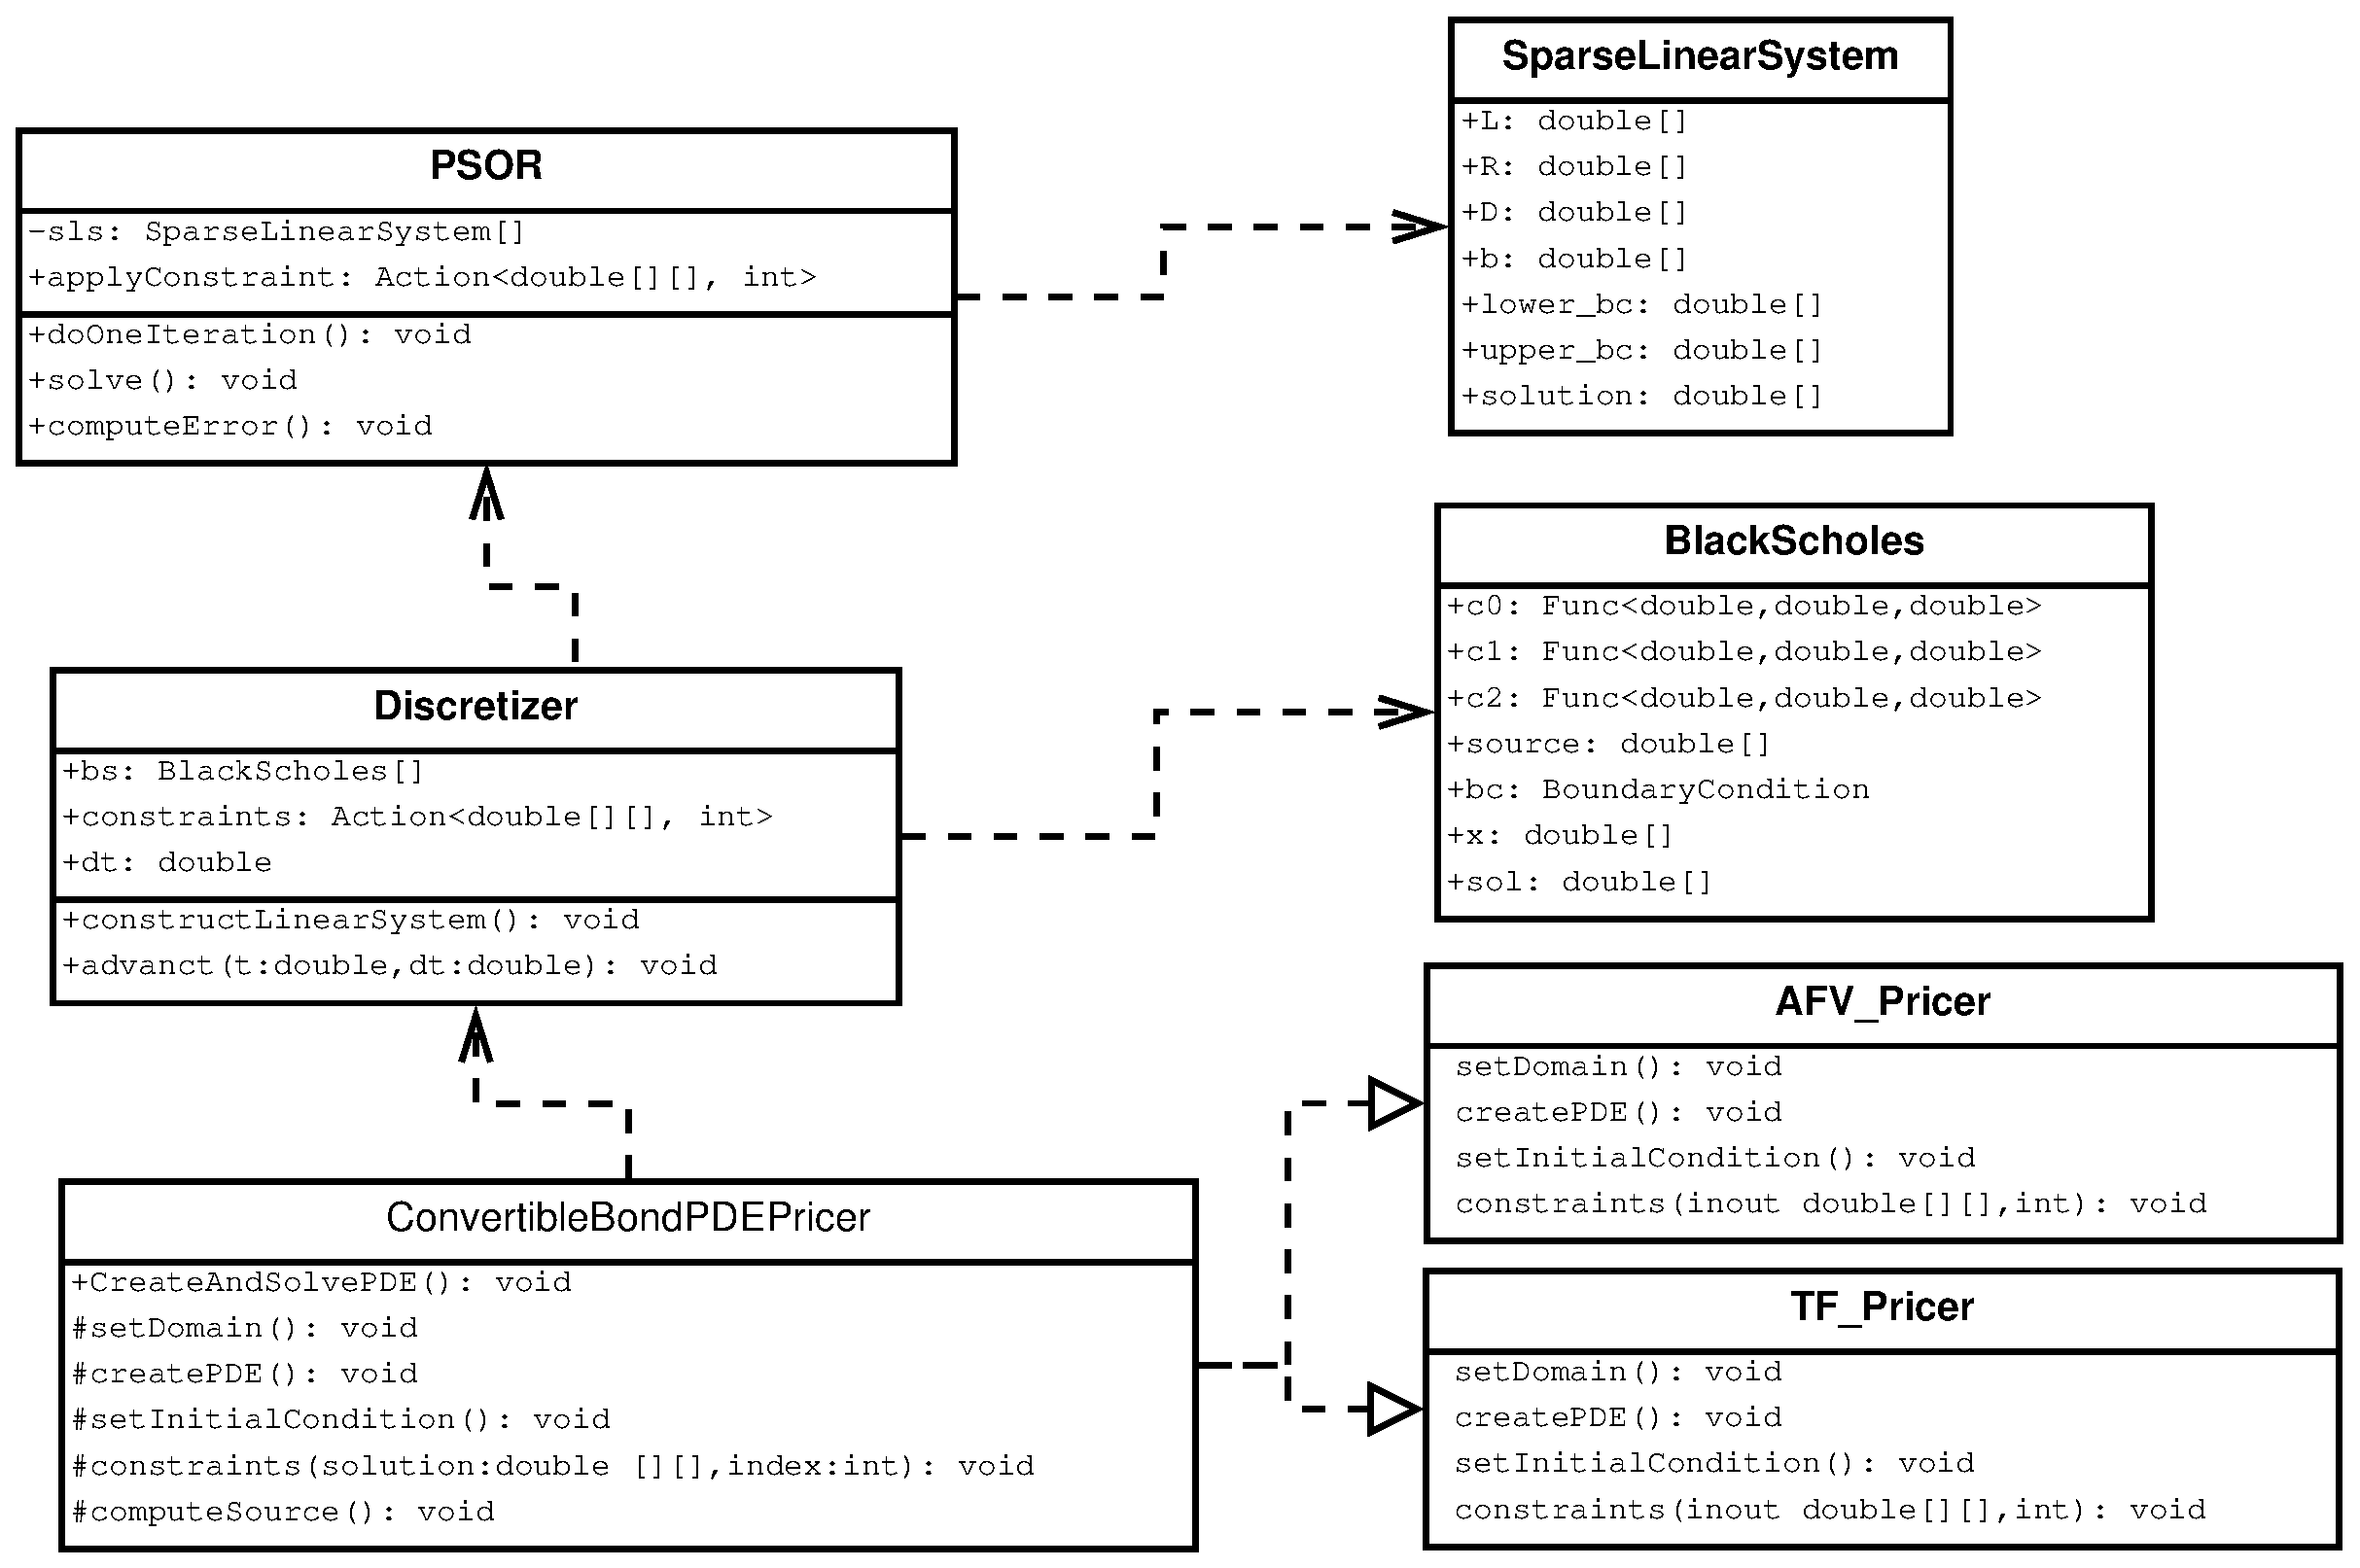
\includegraphics[width=\textwidth]{Figures/CBobjects}
\caption{Interaction between different classes}
\end{figure}
\label{fig:Classes}

\section{Numerical Results}
The algorithm is tested on the convertible bond with the parameters described in Table \ref{tb:params}.
\begin{table}
\centering
\begin{tabular}{ll}
\hline\hline\\
Parameter &  Value \\
\hline\\
Volatility & 0.2 \\
Risk-free interest rate & 0.05\\
Credit risk & 0.02\\
Growth rate of stock & 0.02\\
Time to expiry & 5 \\
Conversion ratio & 1.0 \\
Clean call price & 110 from year 2 to year 5\\
Clean put price & 105 at third year\\
Coupon payments & \$4, semiannually\\
\hline
\end{tabular}
\caption{Parameters for the test case}
\label{tb:params}
\end{table}


The solution for $t = 0$ with different settings are displayed in Figure \ref{fig:compare}. It is obvious that the coupon payments, puttability and callability increase the bond price in different instances.
\begin{figure}[ht]
\centering
\includegraphics[width=0.7\textwidth]{Figures/compare}
\caption{Compare the solution of zero coupon, with put, with call and put}
\label{fig:compare}
\end{figure}

The 3D surface solution for CB and COCB are displayed in Figure \ref{fig:surf}. The coupon payments result in zigzag surface due to their singular formats.
\begin{figure}[ht]
\includegraphics[width=0.49\textwidth]{Figures/CBsurf}
\includegraphics[width=0.49\textwidth]{Figures/COCBsurf}
\caption{Solution surface for CB (left) and COCB (right)}
\label{fig:surf}
\end{figure}

The time cost is almost quadratic $O(N^2)$ on grid size $N$ since increasing the grid size not only increases the computational cost at each time step, but also reduces the time step size in order to maintain a consistent accuracy in both time and space. The relationship between computational time and grid size for the test case is displayed in Figure \ref{fig:time_cost}.
\begin{figure}[ht]
\centering
\includegraphics[width=0.7\textwidth]{Figures/timecost}
\caption{Time cost on computational grid size. The test is performed on both debug version and release version.}
\label{fig:time_cost}
\end{figure}

\end{document}